\chapter{Design}\label{design}

I have chosen to implement a client server model for the system architecture, as this offers a strong separation into multiple loosely coupled modules. Given a client server architecture, and a desire for centralised data storage between multiple users a browser based approach was chosen. Using existing browsers leverages significant work done on secure network communications between client and server, as well as significant effort in sandboxing (isolating from the rest of the computer) in-browser applications. This saves significant time and effort on implementing communication protocols and security.  The client server model was chosen as typical users for the system are expected to be security professionals who can be expected to be required to document and report any abnormal behaviour. The client server model supports sharing the application amongst multiple users. 

As there are relatively few programming languages available for use within the browser this significantly simplified the choice of languages and tool sets. See section \ref{C:impl}.

\begin{figure}[tbh]
\fbox{\parbox[b]{.98\linewidth}{
\vskip 0.5cm
\centering 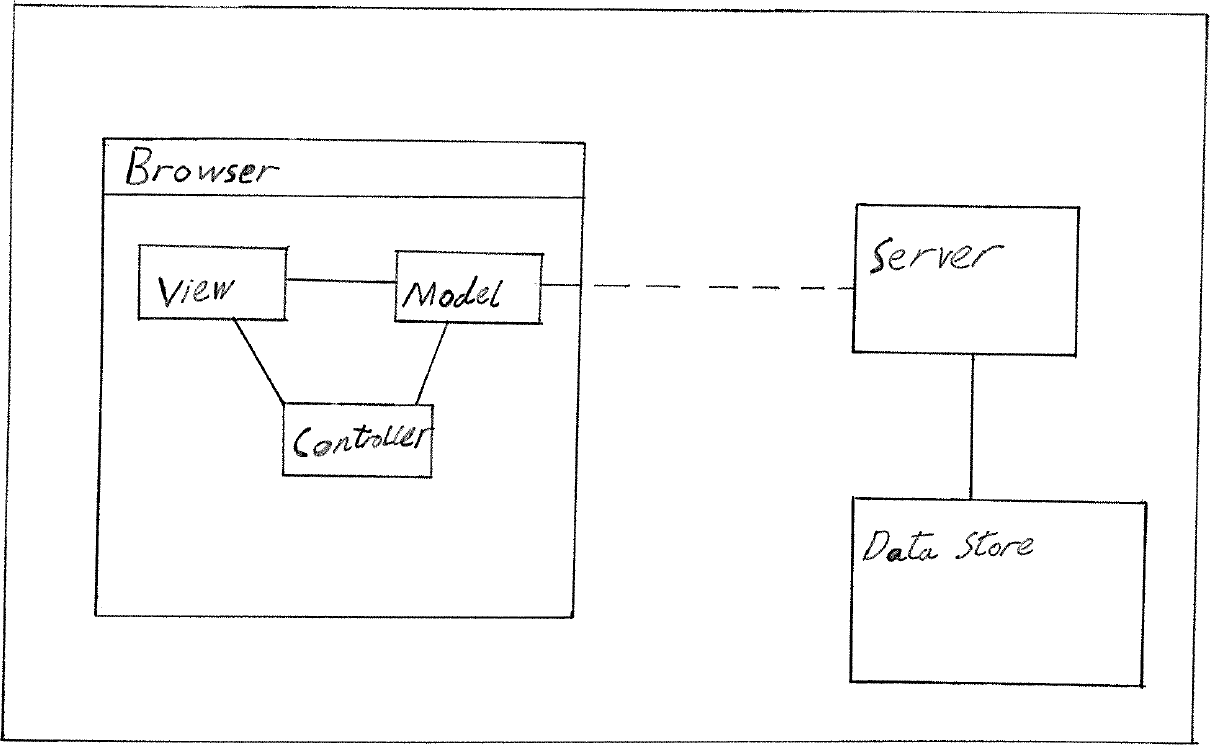
\includegraphics[scale=0.3]{blocks.png}
\vskip 0.5cm}}
\caption{\protect\label{spiral_plan}Block diagram showing proposed architecture of system. Note complete separation between server, browser and datastore. These may reside on separate machines.}
\end{figure}

Inside the browser there are three major components from an object oriented perspective. The view contains what is actually displayed on screen, this is implemented in HTML with SVG (Scalable Vector Graphics) for graphical components. The model stores the data and handles requests to the server as necessary. The controller is responsible for implementing user interaction with the system.

Communication between the client and server is handled through the HTTP protocol, using ajax requests.  The server software is responsible for serving data to the client, performing data aggregation, and limited data mining. In order to provide data, the server communicates with the data-store. This communication uses SQL and the JDBC api to interface with a database. Modular design permits creation of other storage interface modules. 

Data aggregation is performed server side for two reasons. In larger networks or over longer time periods many megabytes of logs can be created. While text is highly compressible this still creates significant network overhead to transfer. Further, there are unanswered questions about how well the client will perform with potentially millions of events to manipulate. Slow data transfers or interaction due to processing time would be a significant usability hurdle. Performing data aggregation on the server bypasses both of these limitations. 

\section{User interface design}\label{screen_design} 
  
I have chosen to adopt a time based approach for the visualisation elements, as access attempt logs have a very strong time component. Some forms of unusual behaviour are evidenced only by unusual times for access attempts, or unusual durations of access for example. Most existing visualisations do not give much emphasis to the time relation between access attempts, preferring to focus on the links between source and destination addresses. 

\subsection{Spiral view}

Spiral view is an approach for displaying time series data mapped to a spiral, see figure \ref{spiral} where a straight line drawn from the outer edge to the center shows the same time at each level of the spiral \cite{bertini2007spiralview, chin2009visual}
These systems appear to be highly effective at displaying time series data in a fashion that supports easy detection of repeated patterns. 

\begin{figure}[tbh]
\fbox{\parbox[b]{0.98\linewidth}{
\vskip 0.5cm
\centering 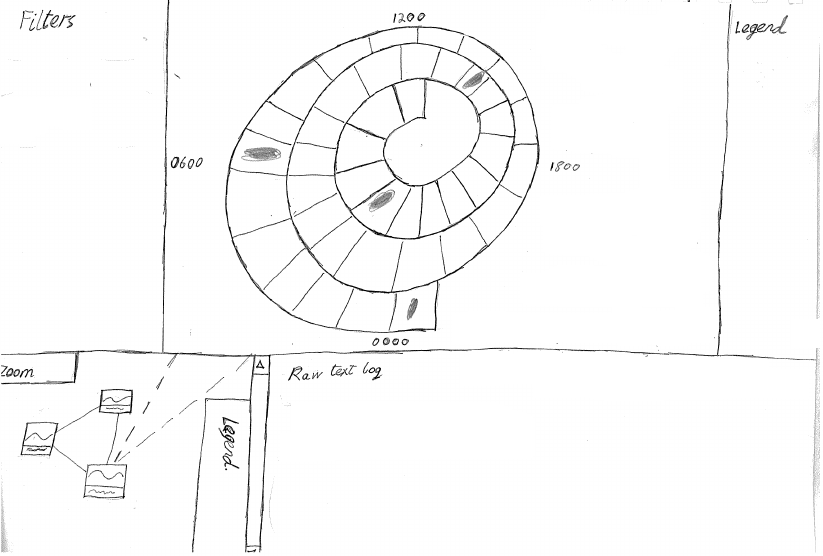
\includegraphics[scale=0.6]{spiral_plan.png}
\vskip 0.5cm }}
\caption{\protect\label{spiral_plan}Drawing showing proposed layout using spiralview for main focus. Black shading shows selection of an event with highlighting of related events.}
\end{figure}
 
However serious flaws in the results(\cite{chin2009visual}) of usability tests presented have lead to the rejection of this method. The error in question shows a table of results that directly contradict claims made in the text about how well spiralview supports the detection of patterns. The claims contradicted in the work are those directly bearing on the uses I had intended for the spiral layout. As this is a 300 hour project, I will not be attempting to repeat their work to clarify their findings. I attempted to contact the authors of the paper, and have as yet received no response.

This contradiction casts doubt on the ability of the spiralview model to effectively support data hiding, navigation and manage potential for information overload. These aspects are key functional requirements for this project \ref{reqs}. Due to this doubt, and lack of response from the authors when clarification was requested, I have chosen not to use the spiral model. 

\begin{figure}[tbh]
\fbox{\parbox[b]{.98\linewidth}{
\vskip 0.5cm
\centering 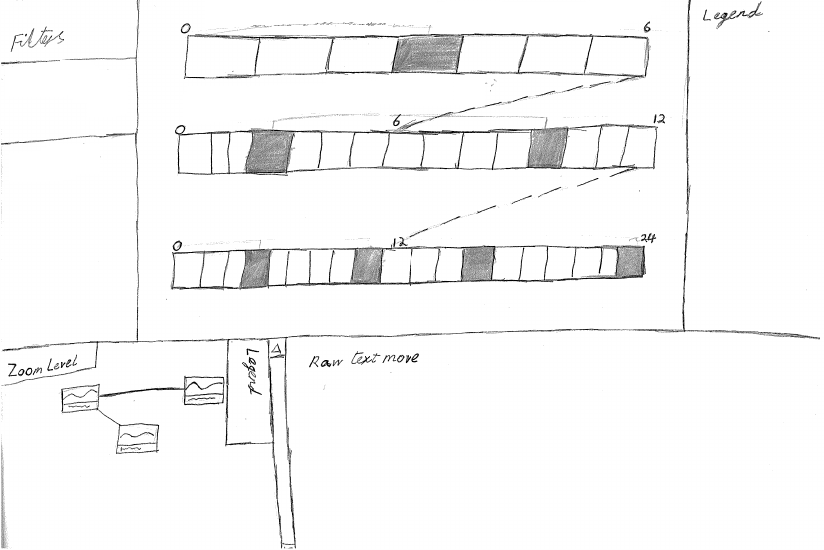
\includegraphics[scale=0.6]{lines.png}
\vskip 0.5cm}}
\caption{\protect\label{lines}Drawing showing proposed layout using multiple time lines for main focus. Black shading shows selection of an event, with highlighting related events.}
\end{figure}

\subsection{Linear Timelines}\label{des_timelines}
Using block representation of data arranged linearly along a time axis.
Initial designs called for using a stacked representation where each layer represented twice the time of the previous layer. This is proposed to show patterns as an element that repeats a growing number of times in each layer.
Tufte's work on small multiples \cite{tufte1983visual} suggests keeping each level of the stack to represent the same amount of time, with differing start and end points. Ie: if the range is 6 hours, the top bar starts at 0600, and runs to 1200, the one below it from 0000 to 0600 and so on. This would show patterns repeating with a period less than the time range by showing in multiple bars. See Figure \ref{lines}. The timeline visualisation chosen is familiar to most people due to wide useage. Familiarity with this model supports information hiding and information overload prevention goals as users can be expected to interpret the timeline structure with minimal cognitive burden. 

I have been forced to consider data hiding techniques, as networks can become extremely busy, producing sufficient activity to overwhelm the user's ability to absorb information and detect meaningful patterns in the clutter. As I have chosen a time series based approach to displaying the data, I have chosen to use time binning to aggregate entities. This approach is extremely simple, with all entries in a short time period displayed as a single entity, with icons indicating some simple features of the hidden data. Such features include superuser accesses, abnormal numbers of failed access attempts, abnormally large numbers of access attempts, abnormal login locations for a user, abnormal login times for a user. Each time bin can be zoomed in on, allowing the user to see greater detail within the bin. For extremely busy systems and longer time periods there may be multiple levels of binning in play to aggregate sufficiently. This scheme reduces the visual complexity, while allowing easy access to detailed information about each incident. 

These last are the most complicated flags, as they require creating a profile of each user's access times over repeated access attempts. This complexity can produce false positives while the system is learning a new user's habits. and may be tripped up by a legitimate change in user habits.

\begin{figure}[tbh!]
\fbox{\parbox[b]{.99\linewidth}{
\centering 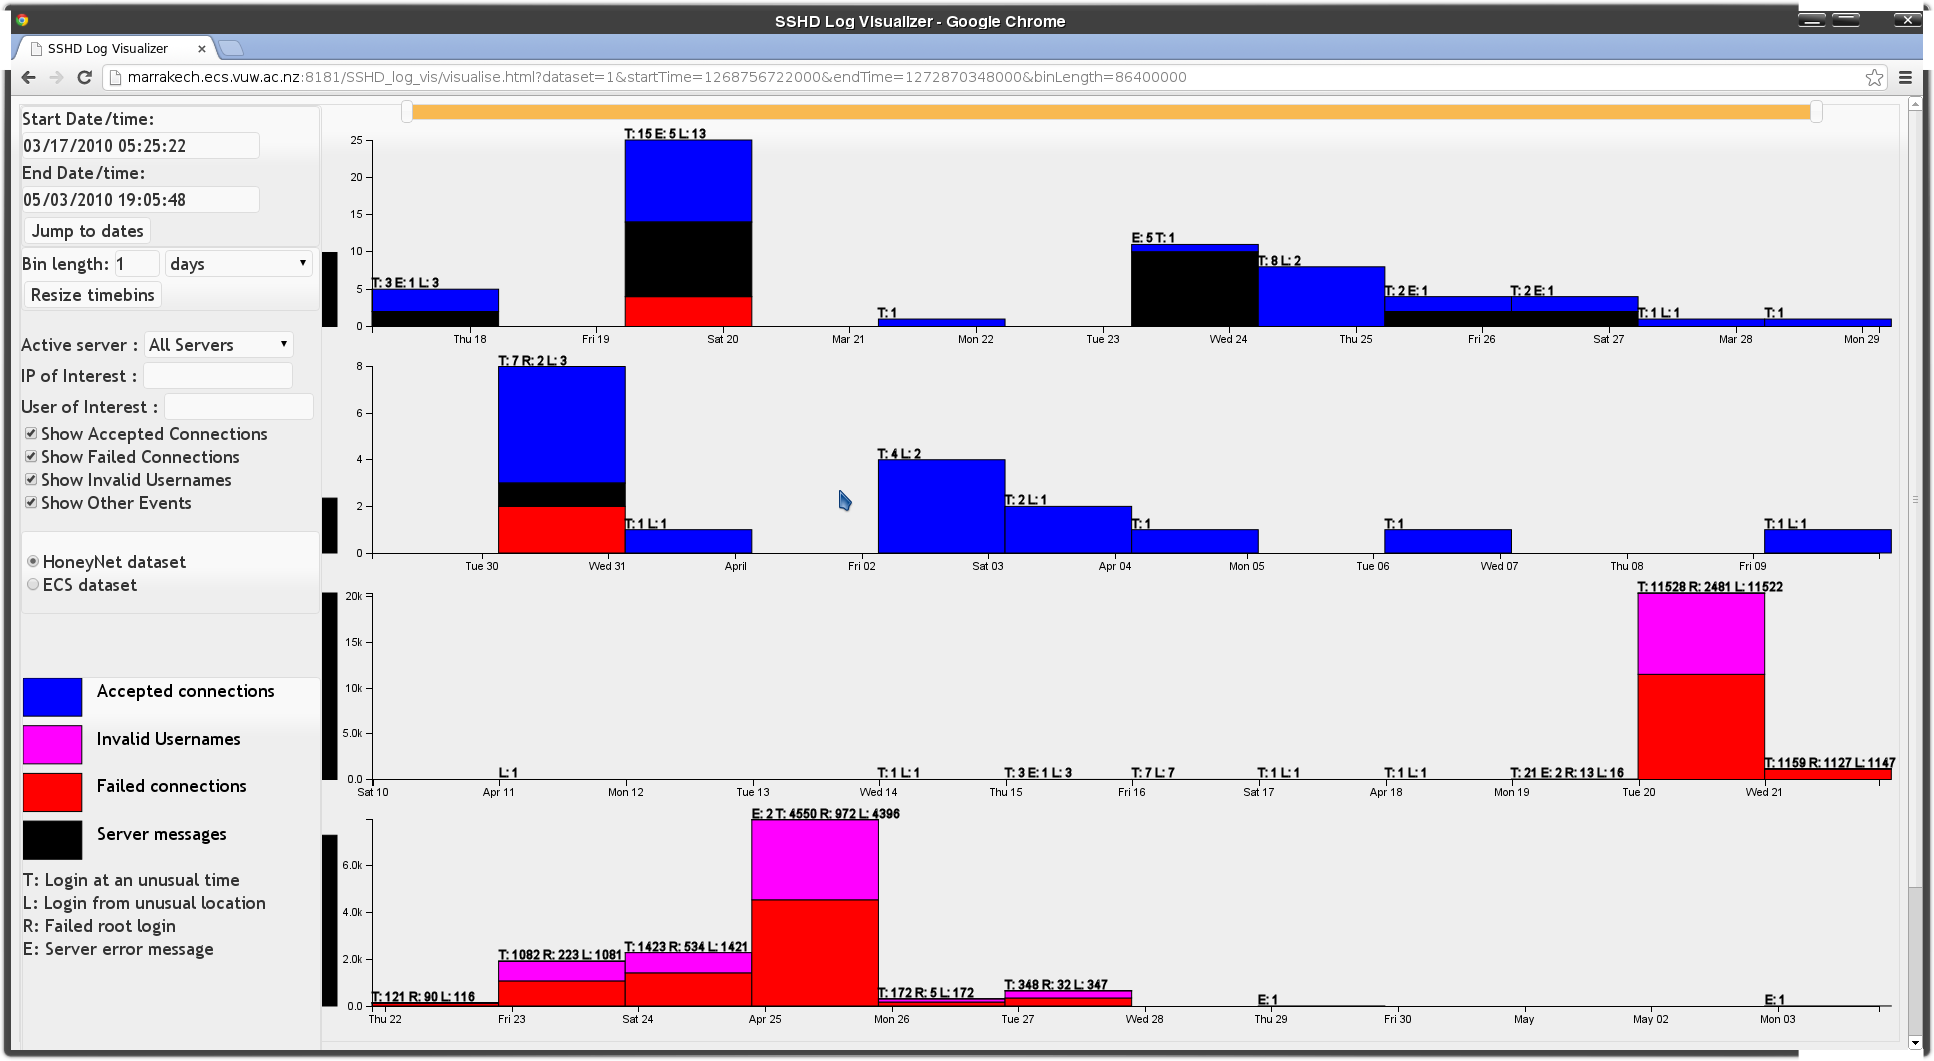
\includegraphics[scale=0.43,  angle=270]{screenshots/overview.png}
}}
\caption{\protect\label{overview}Tool showing overview of the honeynet dataset (\ref{data})}
\end{figure}

\subsection {Final design}

Figure \ref{overview} shows an overview of the tool produced. Network context and Raw line segments were omitted (see \ref{lines}), These two components were considered less important than the timeline visualisations, and as such were dropped due to time pressures.  The space saved by dropping these components allowed more room in the left panel, which has absorbed the legend, allowing the remainder of the screen to be devoted to the timeline view. 

All web application state is stored in the URL, and the application is capable of reloading the state from any correctly formatted URL. This was implemented to support uses expected from the user personae. It is reasonable to expect that a security officer would be required to log information about any detected anomalies, and may wish to obtain a second opinion.
With the tool able to reload state from a URL, this is easily supported simply by passing around the URL via existing collaboration tools, such as email. 
This also allows bookmarking of views that the user finds interesting, for later review or simply as way of saving current progress.  This decision provides a very simple model for supporting sharing and saving requirements (see \ref{reqs}).

Four notable features have been added since the design sketches were produced, vertical scaling; colour-coding of event types; mouseover tooltips; and a timeline overview. 
Within each timeline, blocks are vertically scaled proportional to the block with the largest number of events. Figure \ref{overview} demonstrates this most clearly in the first three blocks of the top timeline. The scale indicates 25 events at maximum, the first block consists of 5 events total, the second block is absent, indicating no events occured in that time, and the third block shows 25 events of three different classes. This was implemented in support of non-functional requirements 1 \& 2, that information hiding be used effectively without masking important data.

Timelines are required to have independent vertical scales as the number of events in a given time period may be highly variable. This is demonstrated in Figure \ref{overview} where the top timeline shows 25 events in the largest bin, and the third shows in excess of 20K events. Without independent scaling for each timeline all features of the upper two lines would be overwhelmed by the third. This lead to the inclusion of the black scale indicators found between the controls and timelines. They are logarithmically scaled such that the timeline with the highest maximum events per bin is represented by a full bar. These provide a quick visual indication of how much variability there is between scales. This supports functional requirement 2, and nonfunctional requirements 1 \& 2.

Each block is subdivided into four colours that represent 4 different classes of log event, as shown in the legend, Each event must be in exactly one event class, this allows the colour sections to be linearly scaled to block height easily (ie: if half the events are failed connections, half of the block will be red). These were added to give an instant overview of the approximate breakdown of event types within each bin, in support of requirements to avoid information overload without masking important data. To further support this goal hovering the mouse over a block produces a tooltip showing a detailed statistical breakdown of the events within that block (see Figure \ref{des_tooltip}). 

\begin{figure}[tbh]
\fbox{\parbox[b]{.99\linewidth}{
\centering 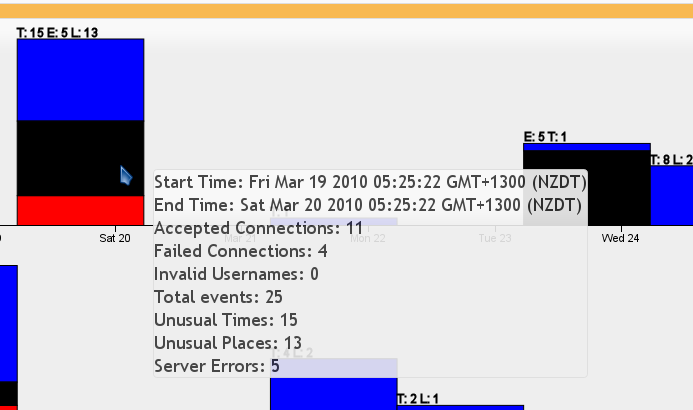
\includegraphics[scale=.35]{screenshots/overview_statistics_cropped.png}
}}
\caption{\protect\label{des_tooltip}Tooltip showing statistics for a block.}
\end{figure}

Above the timelines can be found a slider, when full (as in Figure \ref{overview}) this indicates that the timelines cover all data present. When there is more data off either end the slider shrinks to indicate how long a portion of the dataset is shown. The slider can then be dragged, and will move in steps, each step covering exactly as long as is currently shown in the timelines. Figure \ref{zoomed_in} demonstrates this shrinkage. This slider was added to support navigation through the timeline, as the position of the slider gives an approximate indication of how far through the timeline the view is. The extreme left is when the first log event occured. The extreme right is at the latest log event.

\begin{figure}[tbh!]
\fbox{\parbox[b]{.99\linewidth}{
\centering 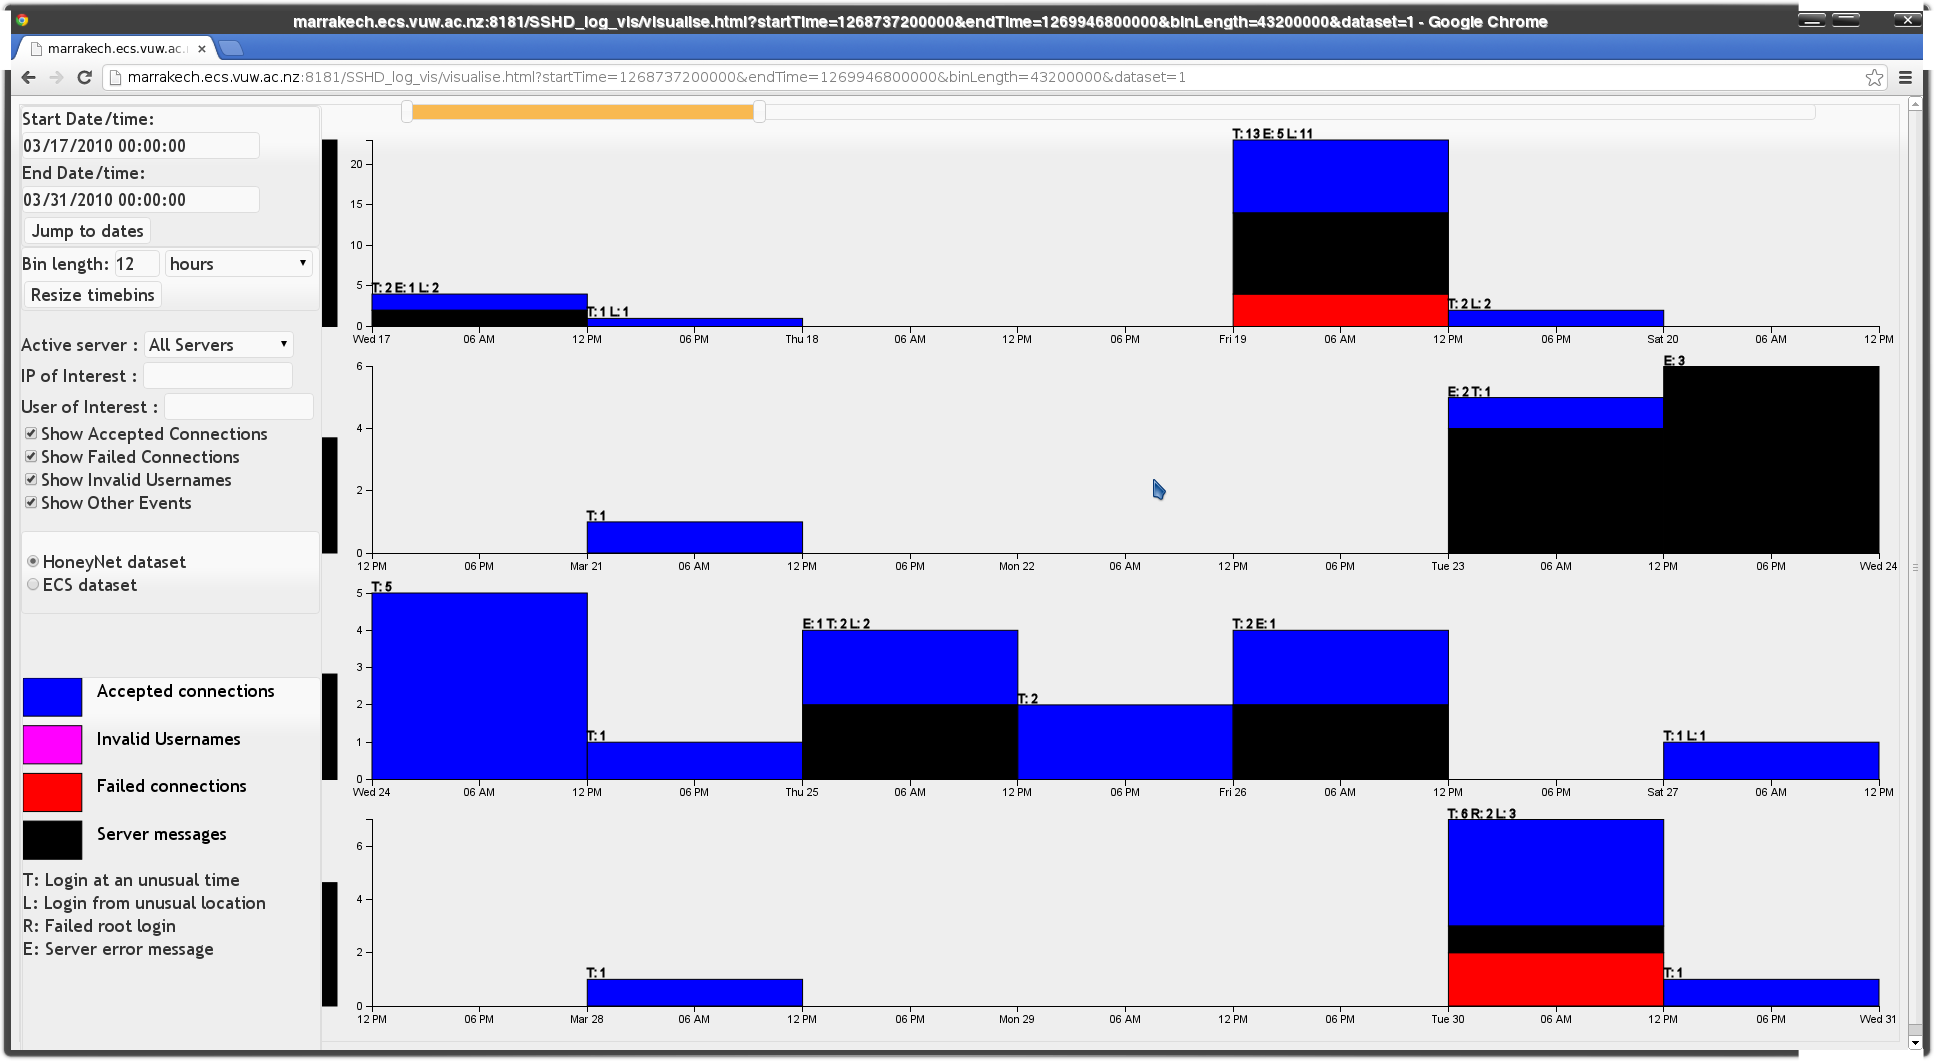
\includegraphics[scale=0.43,  angle=270]{screenshots/2_weeks_zoom.png}
}}
\caption{\protect\label{zoomed_in}Tool showing 2 weeks of Honeynet dataset (\ref{data})}
\end{figure}

Doubleclicking on any block zooms in on that block, with all four timelines reloading to show only data from the selected block. 
Zooming can be performed until either there is only one event in the chosen block, or each block covers 1 second. The one second limit is a practical consideration of the structure of SSHD logs. These logs have a time resolution of 1 second, ie:  all events occuring between 10:59:59.000 and 10:59:59.999 are logged at 10:59:59. Where there is only one event to display, mousing over the block will show the raw log line in a popup. This was implemented to reduce the number of zoom actions required to see details in low activity time blocks.

When there are multiple events in a 1 second block attempting to zoom will produce a popup dialog showing the raw log for that second (Figure \ref{des_one_second}).

\begin{figure}[tbh]
\fbox{\parbox[b]{.99\linewidth}{
\centering 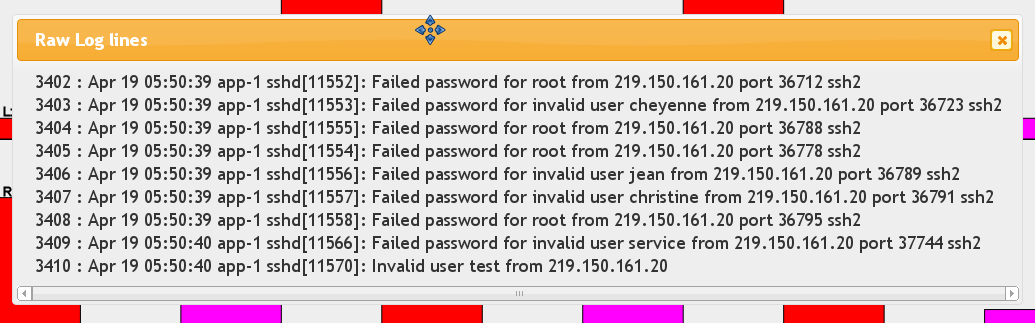
\includegraphics[scale=.35]{screenshots/single_second_popup.png}
}}
\caption{\protect\label{des_one_second}popup showing raw log for a single second.}
\end{figure}

This approach provides an arbitrarily large number of zoom levels, which supports information hiding goals.

No unzoom or undo functions were implemented. Instead the application was integrated with the browser history. This integration gives both undo and redo functions using the browser back and foward buttons. 

\section{Parser}\label{parser}

As SSHD logs are highly structured, this structure largely dictated the structure of the parser. There are 5 major classes of event that can be logged. While there are many more kinds of events, and metadata about connections that can be logged, extended information is highly dependent on SSH demon configuration. The listed message types can be relied on to be present in all useful logging levels. 
\begin{itemize}
\item{Connection attempts}
\item{Disconnection messages}
\item{Subsystem requests}
\item{Invalid usernames}
\item{System messages}
\end{itemize}

All log entries contain a partial timestamp, server name, service name and process id. These fields are required by the syslog format used by openSSH. The remainder of the message is a free text field. Each has different metadata to break down. IE:  a connection attempt has information about authentication method, username, source address, and status. Whereas a disconnection message contains a code, and source IP \ref{log_examples}.

The parser for SSH logs was initially conceived as a monolithic design, with a single class responsible for reading, analysing and writing data to the database. This design lasted into early implementation, where it was abandoned, as it leaves the parser too tightly coupled to the choice of underlying datastore. The parser was seperated into two layers, using a more abstract representation of each possible event type.

\begin{figure}[tbh]
\parbox{.99\textwidth}{
{\small Mar 16 08:25:22 app-1 sshd[4884]: Server listening on :: port 22. \\
Mar 16 08:25:22 app-1 sshd[4884]: error: Bind to port 22 on 0.0.0.0 failed: Address already in use. \\
Apr 19 05:55:20 app-1 sshd[12996]: Accepted password for root from 219.150.161.20 port 55545 ssh2 \\
Apr 19 05:55:20 app-1 sshd[12997]: Invalid user pauline from 219.150.161.20 \\
Apr 19 05:55:21 app-1 sshd[12990]: Failed password for root from 219.150.161.20 port 54890 ssh2 \\
Apr 20 00:00:51 app-1 sshd[24442]: subsystem request for sftp \\
Jun 8 01:03:34 machine0 sshd[1796]: Received disconnect from 38.165.101.19: 11: Bye Bye \\}}
\caption{Examples of SSHD logs, showing each type of message}
\label{log_examples}
\end{figure}

In order to implement the abnormal location and time flags discussed in section \ref{des_timelines} an analysis of login attempts must be performed to detect time and location clusters on a per user basis. This is performed by a simple online algorithm, as the log file may not have an end. Each login attempt is compared with the clusters currently stored in the database, and increments the count of times that location/time has been seen before in the logs. When this is over a threshold defined by the tool user, the login is considered to have occured at a usual time/location.

As user behaviour may change over time, a mechanism has been implemented to expire clusters which have not seen any login attempts for longer than a period defined by the tool user. 

This clustering is performed by the parser, as stable results are required to avoid confusing users. Clustering in the server could only include data in current selection.This would result in instability in results (ie: if select one set of dates, a login is normal, select a different set and it's classified as abnormal). In order to avoid this instability, the server would have to read significantly more of the log for each request, at minumum the expiry period for clusters, and potentially the entire log. This would significantly increase server and datastore loads.

\section{Database} 

A relational database management system (RDBMS) was used as the datastore for this project as they have many advantages for the design of the tool. Concurrent access is handled by all major RDBMS systems, with very high performance. RDBMS systems can be significantly faster than other datastores for complex selection tasks. 

Schema for log events uses a single table to store all types of event \ref{entry_schema}. As there are several subtypes of log events, with differing metadata \ref{parser}, there are many nullable values in the event table.
\begin{table}[tbh]
\centering
\begin{tabular}{l || l | l | p{0.5\textwidth}}
Column & Datatype & Nullable & Conditions \\ \hline
id & Int & No & Autoincremented primary key \\
timestamp & Bigint & No & Timestamp stored as milliseconds since unix epoch. \\
server & int & No & Foreign key, linking to server table. \\
connid & int & No & Badly named, Process id for handling sshd process. \\
reqtype & Enum & No & Tag field, used to identify which of the possible event types this row represents. (connect, disconnect, subystem request, invalid username, other) \\
authtype & Enum & Yes & What authentication method was used. (password, hostbased, key, gssapi, or none) \\
status & Enum & Yes & Did the connection attempt succeed? (accepted, failed) \\
user & int & Yes & Foreign key to user table. \\
source & char(45) & Yes & text representation of Ipv4 or IpV6 address the request originated from. \\
port & smallint & Yes & Port the request was sent from. \\
subsystem & Enum & Yes & Which subsystem was requested. (sftp, scp) \\
code & int & Yes & disconnect code, not actually used. \\
isfreqtime & int & Yes & Reference to information about time cluster this request belongs to, or null. \\
isfreqloc & int & Yes & Reference to information about location cluster this request belongs to, or null. \\
rawline & text & No & Unprocessed line, exactly as read from logfile. \\
\end {tabular}
\caption{Schema for entry table}
\label{entry_schema}
\end{table}

Several considerations were involved in creating this table schema. As there are multiple types of log entry considered by the system, database design suggests three alternative approaches to table layout to handle this. A single unified table, with many nullable elements, A table storing all columns common to each entry type (Non nullable columns in \ref{entry_schema}) with additional tables for each subtype storing only information unique to that entry type. Or a table for each entry type with all attributes used in that subtype, including shared attributes.

It is usually considered good design to avoid large numbers of nullable attributes, as this complicates integrity checking and in many cases forces checks to be carried out at the application level, or in complex stored procedures. However, performance considerations have forced the use of this schema design. In practice, there are very few queries to the database that do not involve a range select on timestamp (all rows with timestamp between x and y) for all subtypes of entry. In both multitable schema designs, this must be implemented with multiple joins (5 or 6). As this tool is intended to scale to many millions of events, and joins are the least efficient database operation, nonfunctional requirements strongly suggest avoiding joins where possible. This has lead directly to the table schema shown \ref{entry_schema}. Note that the server table stores some basic metadata about each server, this is currently not utilized, though may be in future extensions.

The user table started out in an older design, which proposed storing some metadata about users, such as validity, role, and login patterns. This would have eliminated the need for the invalid user request type, as this is just a failed connection, due to invalid user. This design was not pursued, due to issues with time. In the honeynet dataset accounts are created and destroyed. This results in previously invalid usernames becoming valid. With this design, that would require multiple entries for each user, as an invalid user linked against an entry on date x, does not become valid when the user is created on date y (y after x). However this is still necessary for the clustering algorithm implemented in the parser, as each time or location cluster is only valid for a single user. The alternative would be to store the username alongside each cluster. However this would cause difficulties in enforcing uniqueness constraints on usernames, and ensuring consistency between events, and time/location clusters. 

Users may also have several independent frequent login times and locations, ie: Some IT staff may frequently log in from home as well as in the office. This resulted in frequent time and location information being split into four separate tables. <include table schema here?>

\section{Server}
Server implementation was very tightly constrained by choice of platforms. Web applications communicating through the HTTP protocol, with a Tomcat server provide limited opportunities for design choices.
In order for the code to interface with Tomcat, it must be written as at least one class which implements HttpServlet from the java API. 
This class serves to handle communication with the Tomcat server. Tomcat provides HTTP request parsing, session tracking and multithreading. Further classes may be used freely to implement servlet behaviour. As very simple behaviour is required from the server, I chose to use a two layer architechture for each Servlet. 
\begin{itemize}
\item{Data access layer. Responsible for fetching data from the underlying datastore. easily replaced to communicate with different kind of datastore. Takes values from client communication layer, returns lists of matching log entries.}
\item{Client Communication layer. Responsible for aggregating data returned by the data access layer, and building HTTP responses from the aggregated data. Including JSON translation.}
\end{itemize}
The data access layer is common to all servlets, and has a defined interface, with methods for fetching data to satisfy each type of request. This design allows for substitution of a different data storage system with minimal changes to the system. Servlets would need to be modified only to instantiate the new data access layer when initialised. This could be easily modified to use a static factory method, which would further restrict the area requiring changes.

There are exactly 4 types of request that may be made of the server, The majority of requests made in normal usage will be requests for aggregated events. 
\begin{itemize}
\item{Request aggregated events between given timestamps, and optional filters on username, server, and source IP}
\item{Request raw events between given timestamps, and optional filters on username, server, and source IP}
\item{Request start and end timestamps}
\item{Request list of all servernames}
\end{itemize}

These four requests to the server, are implemented with three requests to the underlying datastore.

\begin{itemize}
\item{Fetch log lines - used to fetch all log lines between a given pair of timestamps, with optional filters on username, server, and source IP}
\item{Fetch start and end times - used to fetch the timestamps of the first and last events in the datastore}
\item{Fetch all server names - used to fetch a list of every server name known to the datastore}
\end{itemize}

All request types are independent servlets within the web application. Each servlet has no shared state, so parallelizes easily within the tomcat framework. Connection pooling is implemented to assist in performance where multiple users may be requesting data. Concurrent read/write issues are the responsibility of the underlying datasource.

The first two request types use the same interface to the datasource, but have differing post processing applied. raw does not do any agreggation, simply converts the data into JSON format and embeds in the HTTP response. aggregated collects statistics about all events which fall in that time period, statistics are transmitted in JSON format as payload of HTTP response.
Why have aggregated request? nonfunctional requirements - performance and data hiding. aggregation done serverside due to bandwidth and memory requirements, this operation could involve processing millions of nodes for larger logs. This is unreasonable to send across the network in raw form, due to size and space requirements. Server has resources to do aggregation. 
some room for refactoring, this could be split into two layers
however the processing is quite simple, and only done for this one request type, so a data analysis layer was omitted.

\subsection{Security}

The database will contain a significant amount of privileged information about network security such as machine names and addresses, valid account names, and authentication methods used in the system. This data would be extremely useful to malicious users or outside intruders. 

As the tool is accessed through the browser there are concerns about the security of this information. As implemented, the tool does not directly include any authentication or access control mechanisms. However, the server is written to be resistant to SQL injection attacks through rigorous input sanitation.

This leads to a need to ensure that access to this tool is controlled through a robust authentication system. Ideally the web server hosting the tool should not be accessible to the outside world at all. Further, access should be restricted tightly to only those users with a definite need to have access. Secured connections must be used for all communication between client and server to limit the opportunity for malicious individuals to snoop on the data in transit. Tomcat natively supports access controls on a per application, or per page basis. Tomcat also supports SSH connection, and can be configured to require SSH connections on a per page or per app basis. These controls are managed through tomcat configuration files. 

Client side code contains no data, and so does not require security, as the server should deny access without valid credentials.